\documentclass{standalone}
\usepackage{tikz}

\tikzset{
    box/.style={
        rectangle,
        draw,
        fill=gray!20,
        rounded corners,
        minimum height=0.8cm,
        text width=3cm,
        align=center
    },
    bluebox/.style={
        box,
        fill=blue!20
    },
    redbox/.style={
        box,
        fill=red!20
    }
}

\begin{document}
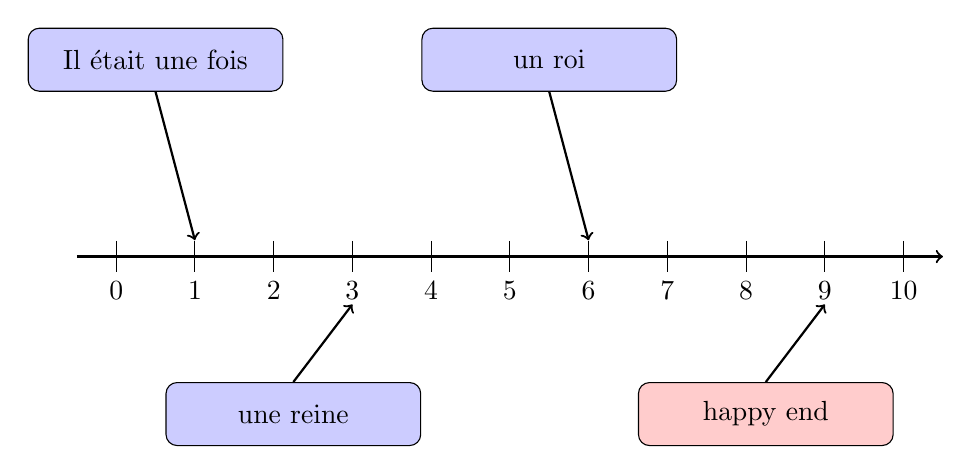
\begin{tikzpicture}
    \draw[->, thick] (-0.5, 0) -- (10.5, 0);
    \foreach \x in {0,1,...,10} {
        \draw[-] (\x, 0.2) -- (\x, -0.2) node[below] {\x};
    }

    \node[bluebox] (fois) at (0.5, 2.5) {Il était une fois};
    \node[bluebox] (reine) at (2.25, -2) {une reine};
    \node[bluebox] (roi) at (5.5, 2.5) {un roi};
    \node[redbox] (fin) at (8.25, -2) {happy end};

    \node[inner sep=0.2cm] (foisinstant) at (1, 0) {};
    \node[inner sep=0.6cm] (reineinstant) at (3, 0) {};
    \node[inner sep=0.2cm] (roinstant) at (6, 0) {};
    \node[inner sep=0.6cm] (fininstant) at (9, 0) {};

    \draw[->, thick] (fois.south) -- (foisinstant.north);
    \draw[->, thick] (roi.south) -- (roinstant.north);
    \draw[->, thick] (reine.north) -- (reineinstant.south);
    \draw[->, thick] (fin.north) -- (fininstant.south);

\end{tikzpicture}
\end{document}
